\chapter{Weitere topologische Begriffe}\label{chap:topologie-erweiterung}

In diesem Kapitel definiere ich eigene Begriffe auf topologischen Räumen, die ich für die formale Definition der \strukt benötige.
Dazu gehören:
\begin{enumerate}
    \item die \textemph{lokale Gleichheit} als Grundlage für die Definition der Objektäquivalenz
    \item \textemph{einfache Mengen} als Kandidaten für Raumregionen sowie euklidische Flächen und Linien
    \item der \textemph{äußere Rand}: euklidische Flächen, Linien und Punkte sind ausgewählte Teilmengen des äußeren Randes.
\end{enumerate}
%Außerdem werden in Abschnitt \ref{ssec:notationelle-konv} vereinfachte Notationen für oft gebrauchte Operatoren eingeführt.


    
                            %%%%%%%%%%%%%%%%%%%%%%%%%%
                          %%%                        %%%
%%%%%%%%%%%%%%%%%%%%%%%%%%%      Lokale Gleichheit      %%%%%%%%%%%%%%%%%%%%%%%%%%%%%%%%%%
                          %%%                        %%%
                            %%%%%%%%%%%%%%%%%%%%%%%%%%


\section{Lokale Gleichheit}\label{sec:lokale-gleichheit}
    Zwei
    \marginpar{lokale Gleichheit}
    Flächenrepräsentanten sollen objektäquivalent sein, 
    wenn sie koinzidieren und die Raumregionen, die sie begrenzen \glqq von der gleichen Seite kommen\grqq. 
    Analoges gilt für Linien- und Punktrepräsentanten. 
    Der Begriff der lokalen Gleichheit ist ein Ansatz, formal zu beschreiben, was es heißt, \glqq von der gleichen Seite\grqq\ zu kommen.
    
    Anschaulich gesprochen sind zwei Teilmengen eines topologischen Raumes dann lokal gleich bezüglich eines Punktes, wenn dieser eine Umgebung hat, in der sie nicht zu unterscheiden sind.
    Sie sind lokal gleich bezüglich einer Menge, wenn sie lokal gleich sind bezüglich jeden Punktes dieser Menge.
%    
%     Eine anschauliche Vorstellung dieses Begriffs lässt sich durch das Ameise-im-Nebel-Bild beschreiben:\\
%     Eine Ameise kann sich innerhalb einer Fläche $B$ frei bewegen. Sie kann in alle Richtungen sehen, aber nur ein kleines Stück, denn es herrscht dichter Nebel. Dieser Nebel ist möglicherweise unterschiedlich dicht an verschiedenen Stellen. Zwei Raumregionen $A_1$ und $A_2$ sind lokal gleich bzgl. $B$, wenn es einen \glqq Nebel\grqq\ gibt, so dass die Ameise $A_1$ und $A_2$ nicht unterscheiden kann.
%
    \begin{dfn}[Lokal gleich]\label{def:lok-gleich}\ \\
        Seien $X$ ein topologischer Raum, $A_1, A_2 \subseteq X$.
        $A_1$ und $A_2$ sind \thmemph{lokal gleich} 
        \begin{itemize}
            \item in einem Punkt ${p \in X}$, falls es ein ${U \in \offen(p)}$ gibt mit \\
            ${U \cap A_1 = U \cap A_2}$.
            \item bzgl. einer Menge $M \subseteq X$, falls $A_1$ und $A_2$ in jedem Punkt von $M$ lokal gleich sind.
        \end{itemize}
        Wir schreiben ${A_1 =_x A_2}$, falls $A_1$ und $A_2$ lokal gleich sind in bzw. bzgl. $x$.
    \end{dfn}
%    
    \begin{bem}\ \\
     In einem metrischen Raum lässt sich lokale Gleichheit in einem Punkt $p$ äquivalent definieren durch:
     $$ A_1 =_p A_2 \quad \quad \Leftrightarrow \quad \quad \exists\: \varepsilon > 0 : B_\varepsilon(p) \cap A_1 = B_\varepsilon(p) \cap A_2.$$
    \end{bem}
%    
    \begin{bsp}\label{bsp:lok-gleich}\ \\
     $A_1 := (0,1)^2$ und $A_2 := (0,2) \times (0,1)$ sind lokal gleich bzgl. $M_1 := (0,1) \times \{0\}$ nicht jedoch bzgl. $M_2 := [1,2] \times \{1\}$, denn für jeden Punkt $p_1 = (x_1,0)$ ist mit $\varepsilon_1 := min\{x_1,1-x_1\}$ $B_{\varepsilon_1/2}(p_1)$ eine Umgebung von $p_1$ auf der sich $A_1$ und $A_2$ nicht unterscheiden.
     Aber für $(1,1) \in M_2$ gibt es keine Umgebung $U$ mit $U \cap A_1 = U \cap A_2$ (siehe Abbildung \ref{fig:lok-gleich}).
    \end{bsp}
%    
    \begin{figure}[ht]
        \centering
        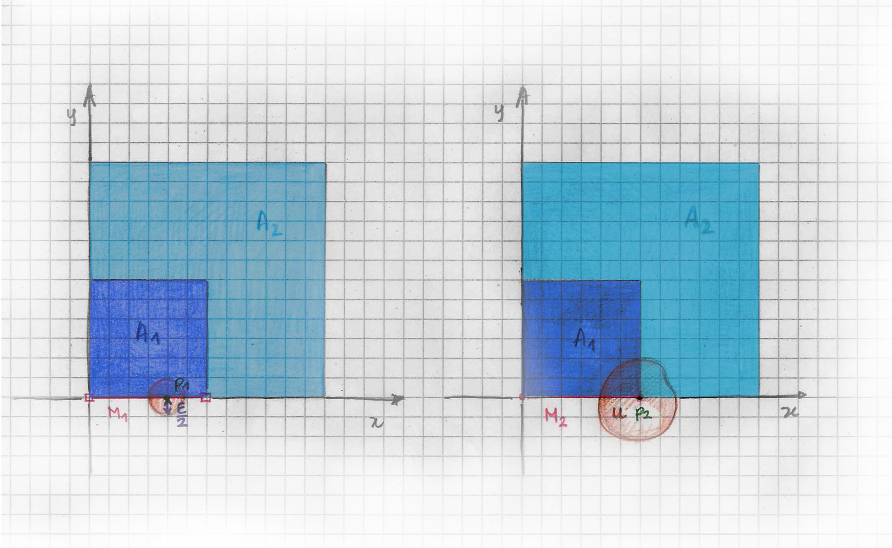
\includegraphics[width=\textwidth]{abb/lok-gleich.png}
        %\caption[Lokale Gleichheit]{Zu Beispiel \ref{bsp:lok-gleich}}
        \caption{Zu Beispiel \ref{bsp:lok-gleich}}
        \label{fig:lok-gleich}
    \end{figure}
%
    \begin{satz}\label{satz:lokale-gleichheit-aer}
        Die lokale Gleichheit in einem Punkt ist eine Äquivalenzrelation.\\
        (Beweis: siehe Anhang \ref{anh:lokale-gleichheit-aer})
    \end{satz}
%  
    \begin{kor}\label{kor:lokale-gleichheit-aer}
     Die lokale Gleichheit bzgl. einer festen Menge ist eine Äquivalenzrelation.\\
     (Beweis: direkte Folgerung aus dem vorhergehenden Satz.)
    \end{kor}
%    
    Die folgenden Sätze besagen, dass lokal gleiche Mengen auch lokal die gleichen Randpunkte haben.
%
    \begin{satz}\label{satz:rand-lokal-gleich}\ \\
        Seien $X$ ein topologischer Raum, $p \in X$, $A,B \subseteq X$ mit $A =_p B$. Falls $p \in \rand A$ ist, so ist $p$ auch in $\rand B$.\\
        (Beweis: siehe Anhang \ref{anh:rand-lokal-gleich})
    \end{satz}
%  
    \begin{kor}\ \\ 
        Seien $X$ ein topologischer Raum, $A_1, A_2 \subseteq X$, $B \subseteq \rand A_1$, $A_1 =_{B} A_2$. Dann ist $B \subseteq \rand A_2$.\\
        (Beweis: direkte Folgerung aus dem vorhergehenden Satz.)
    \end{kor}
%     \todo[inline]{FL: Ich hoffe, die Korrektur zweier Auftreten von $B_1$ zu $B$ ist korrekt.\\
%     -> BH: bestimmt!}


    
    
                            %%%%%%%%%%%%%%%%%%%%%%%%%
                          %%%                       %%%
%%%%%%%%%%%%%%%%%%%%%%%%%%%      Einfache Mengen      %%%%%%%%%%%%%%%%%%%%%%%%%%%%%%%%%%
                          %%%                       %%%
                            %%%%%%%%%%%%%%%%%%%%%%%%%

\section{Einfache Mengen}\label{sec:einf-mengen}

    Einfache Mengen werden die Kandidaten für Raumregionen, euklidische Flächen und Linien sein.
    In Abschnitt \ref{sec:zusammenfassung} wurden einige wünschenswerte Eigenschaften dieser Objekte zusammengefasst.
    Wie wir im Folgenden sehen werden, schließen einfache Mengen einige offensichtlich unerwünschte Fälle aus. 
    Ob sie ausreichend sind, um alle gewünschten Eigenschaften zu gewährleisten, bleibt noch zu untersuchen (vgl.\ Abschnitt \ref{sec:offene-fragen}).


\subsection{Definitionen und Eigenschaften}
%     \todo[inline]{FL: Alternative Überschrift: Charakterisierung\\
%     Überschrift eingefügt, um die einzelne Überschrift '5.2.1 Ein Beispiel' zu vermeiden, da in aller Regel mind.\ zwei Unterüberschriften genutzt werden, wenn überhaupt untergliedert wird.\\
%     - BH: ``Definitionen und Eigenschaften'' finde ich OK}
    In
    \marginpar{maximaldimensional}
    unserer Vorstellung sind Raumregionen überall dreidimensional (R1). D.h. insbesondere, sie haben keine \glqq niederdimensionalen Ausläufer\grqq.
    Eingebettet in einen dreidimensionalen Raum sind Raumregionen also maximaldimensionale Teilmengen.
%
    \begin{dfn}[Maximaldimensional]\label{def:maxdim}\ \\
        Sei $X$ ein topologischer Raum. Eine Teilmenge $A \subseteq X$ heißt \thmemph{maximaldimensional}, wenn für jeden Punkt $a \in A$ gilt:
        $$\forall\: U \in \offen_X(a) : U \cap \op_X(A) \neq \varnothing$$ 
    \end{dfn}
%    
%    
    Die folgenden Sätze geben zwei einfach zu zeigende Eigenschaften für maximaldimensionale Mengen an, die in einigen Beweisen genutzt werden.
%
    \begin{satz}\label{satz:offen-maxdim}
        Jede offene Menge ist maximaldimensional.\\
        (Beweis: trivial)
    \end{satz}
%    
%    
    \begin{satz}\label{satz:abschluss-maxdim}
        Der Abschluss jeder maximaldimensionalen Menge ist maximaldimensional.
    \end{satz}
%    
    \begin{bew}
        Sei $A$ maximaldimensional. 
        Angenommen $\cl(A)$ ist nicht maximaldimensional.
        Dann gibt es ein $x \in \cl(A)$ und eine offene Umgebung $U \in \offen(x)$, s.d. $U \cap \op(cl(A)) = \varnothing$ ist.
        Dann ist natürlich auch $U \cap \op(A) = \varnothing$.
        Da $A$ maximaldimensional ist, muss dann auch $U \cap A = \varnothing$ sein, denn falls es eine $y$ in $U \cap A$ gäbe, wäre $U$ auch eine offene Umgebung von $y \in A$ und somit müsste $U \cap \op(A) \neq \varnothing$ sein.
        Damit kann $x$ nicht in $\cl(A)$ sein. 
        $\lightning$
    \end{bew}
%
%
    Die folgenden drei Beispiele zeigen maximaldimensionale und nicht maximaldimensionale Mengen im $\R^2$.
%
    \begin{bsp}\label{bsp:maximaldimensional-1}
        $A := \{(x,y) \in \R^2 \mid x^2 \leq y\} \subseteq \R^2$ ist maximaldimensional.
    \end{bsp}
%
    \begin{bew}
        Sei $(a,b) \in A$. Sei $U \in \offen((a,b))$. Sei $\varepsilon > 0$ mit $B_\varepsilon((a,b)) \subseteq U$. Dann ist $(a,b+\varepsilon) \in U \cap \op(A)$.
    \end{bew}
%
%    
    \todo[inline]{Bilder zu den Beispielen zusammenfassen}
    \begin{figure}[ht]
        \centering
        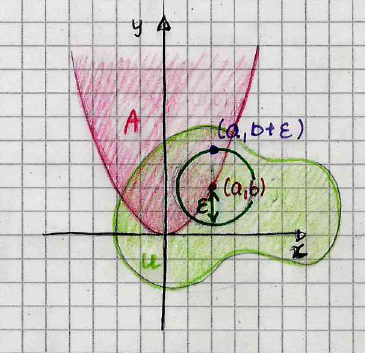
\includegraphics[width=5cm]{abb/maxdim-1.png}
        \caption{Zu Beispiel \ref{bsp:maximaldimensional-1}}
        \label{fig:maxdim-1}
    \end{figure}
%
    \begin{bsp}\label{bsp:maximaldimensional-2}
        $B := \{(x,y) \in \R^2 \mid x^2 \leq y\} \setminus \{0\} \times \R \subseteq \R^2$ ist maximaldimensional.
    \end{bsp}
%
    \begin{bew}
        Sei $(a,b) \in B$. Sei $U \in \offen((a,b))$. Sei $\varepsilon > 0$ mit $B_\varepsilon((a,b)) \subseteq U$. Dann ist $(a,b+\frac{\varepsilon}{2}) \in U \cap \op(B)$.
    \end{bew}
%
%    
    \begin{figure}[ht]
        \centering
        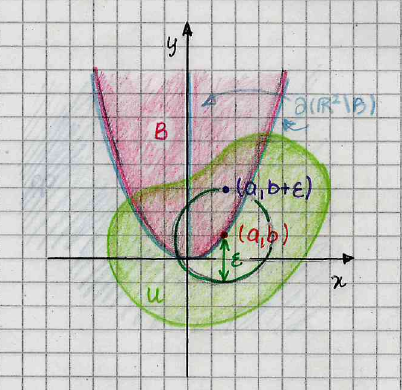
\includegraphics[width=5cm]{abb/maxdim-2.png}
        %\caption[Maximaldimensionale Menge]{Zu Beispiel \ref{bsp:maximaldimensional-2}}
        \caption{Zu Beispiel \ref{bsp:maximaldimensional-2}}
        \label{fig:maxdim-2}
    \end{figure}
%
    \begin{gegenbsp}\label{gegenbsp:maximaldimensional}
        $C := \{(x,y) \in \R^2 \mid x^2 \leq \max\{0,y\}\} \subseteq \R^2$ ist nicht maximaldimensional.
    \end{gegenbsp}
%
    \begin{bew}
        Mit $A$ aus Bsp. \ref{bsp:maximaldimensional-1} sind $C = A \cup \{0\} \times \R$ und $\op(C) = \op(A) = \{(x,y) \in \R^2 \mid x^2 < y\}$. Also ist $(0,-2) \in C$, aber für $U := B_1((0,-2))$ ist $U \cap \op(C) = \varnothing$.
    \end{bew}
%
%    
    \begin{figure}[ht]
        \centering
        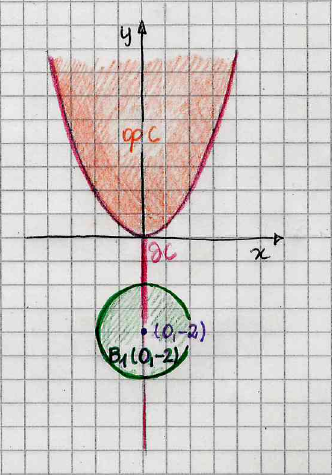
\includegraphics[width=5cm]{abb/nicht-maxdim.png}
        %\caption[Nicht-maximaldimensionale Menge]{Zu Beispiel \ref{gegenbsp:maximaldimensional}}
        \caption{Zu Beispiel \ref{gegenbsp:maximaldimensional}}
        \label{fig:nicht-maxdim}
    \end{figure}
%
    Obige
    \marginpar{Probleme mit maximaldimensionalen Mengen}
    Beispiele legen nahe, dass maximaldimensionale Mengen in $\R^n$ keine niederdimensionalen Ausläufer haben können.
    Sie können jedoch immer noch niederdimensionale Löcher aufweisen.
    Einfache Mengen im $\R^3$ können beispielsweise Kurven als Löcher haben und somit Randstücke, die nicht 2-dimensional sind, wie in (R2) gefordert. 
    Beispiel \ref{bsp:maximaldimensional-2} beschreibt eine 2-dimensionale Menge mit einem 1-dimensionalen Loch.
    
    Beispiel \ref{bsp:maximaldimensional-2} zeigt ein weiteres Problem, das in den Forderungen (R0) - (R2) nicht thematisiert wird. Diese Menge hat einen \glqq inneren\grqq\ Rand. Die positive $y$-Achse ist Rand der Menge $B$, obwohl $B$ sowohl links als auch rechts dieser Achse liegt. Für eine Linienregion, die Teil dieser Geraden ist, würde das bedeuten, dass nicht klar ist \glqq von welcher Seite\grqq die Flächenregion kommt, die sie begrenzt.
    
    Um
    \marginpar{einfache Menge}
    solche Fälle auszuschließen, soll auch das Komplement einer einfachen Menge maximaldimensional sein.
%
    \begin{dfn}[Einfache Menge, $\einf$, $\CO_X$, $\OC_X$]\label{def:einf}\ \\
        Sei $X$ ein topologischer Raum. Eine Teilmenge $A \subseteq X$ heißt 
        \begin{enumerate}
            \item \thmemph{einfach}, wenn sie und ihr Komplement $X \setminus A$ maximaldimensional sind,
            \item \thmemph{einfach abgeschlossen}, wenn sie einfach ist und abgeschlossen,
            \item \thmemph{einfach offen}, wenn sie einfach ist und offen.
        \end{enumerate}
        Die \thmemph{Menge der einfachen Mengen} in $X$ bezeichnen wir mit $\einf_X$, die der \thmemph{einfach abgeschlossenen Mengen} mit $\CO_X$ und die der \thmemph{einfach offenen Mengen} mit $\OC_X$.\\
        Wenn dies nicht zu Uneindeutigkeit führt, schreiben wir auch $\einf$, $\CO$ und $\OC$.
    \end{dfn}
%
%
    Wie sieht es nun mit der Einfachheit der obigen Beispiele aus?
%
    \begin{bsp}\label{bsp:einfach}
        $A = \{(x,y) \in \R^2 \mid x^2 \leq y\}$ aus Bsp. \ref{bsp:maximaldimensional-1} ist einfach.
    \end{bsp}
%
    \begin{bew}
        Klar ist: $A$ ist maximaldimensional. Da $A$ abgeschlossen ist, ist ihr Komplement offen und somit auch maximaldimensional.
    \end{bew}
%
%
    \begin{gegenbsp}\label{gegenbsp:einfach-1}
        $B = \{(x,y) \in \R^2 \mid x^2 \leq y\} \setminus \{0\} \times \R$ aus Bsp. \ref{bsp:maximaldimensional-2} ist \textit{nicht} einfach.
    \end{gegenbsp}
%
    \begin{bew}
        $B$ ist zwar maximaldimensional, aber $\R^2 \setminus B = \{(x,y) \in \R^2 \mid x^2 > y\} \cup \{0\} \times \R$ und somit ist $(0,2) \in \R^2 \setminus B$, aber $B_1((0,2)) \cap \op(\R^2 \setminus B) = B_1((0,2)) \cap \{(x,y) \in \R^2 \mid x^2 > y\} = \varnothing$.
    \end{bew}
%
    \begin{figure}[ht]
        \centering
        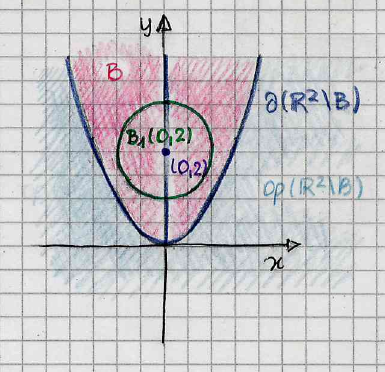
\includegraphics[width=5cm]{abb/nicht-einfach.png}
        %\caption[Nicht-einfache Menge]{Zu Beispiel \ref{gegenbsp:einfach-1}}
        \caption{Zu Beispiel \ref{gegenbsp:einfach-1}}
        \label{fig:nicht-einfach}
    \end{figure}
%
%
    \begin{gegenbsp}\label{gegenbsp:einfach-2}
        $C = \{(x,y) \in \R^2 \mid x^2 \leq \max\{0,y\}\}$ aus Gegenbsp. \ref{gegenbsp:maximaldimensional} ist nicht einfach, da nicht maximaldimensional.
    \end{gegenbsp}
%
    Diese Beispiele legen nahe, dass einfache Mengen in $\R^n$ auch keine niederdimensionalen Löcher haben können.
    
    Die folgenden Sätze geben Eigenschaften von einfachen Mengen an, die für Beweise nützlich sein können.
%
    \begin{satz}\label{satz:einf-komplement}
        Sei $X$ ein topologischer Raum. Eine Teilmenge $A \subseteq X$ ist genau dann einfach, wenn ihr Komplement einfach ist.\\
        (Beweis trivial.)
    \end{satz}
%    
%    
    \begin{satz}\label{satz:inneres-einf-offen}
        Das Innere jeder einfachen Menge ist einfach offen.
    \end{satz}
%    
    \begin{bew}
        Sei $X$ eine topologischer Raum, $A \in \einf_X$. 
        Klar: $\op(A)$ ist offen und als offene Menge nach Satz \ref{satz:offen-maxdim} maximaldimensional.
        Zu zeigen ist also noch: $X \setminus \op(A)$ ist maximaldimensional.
        Da $A \in \einf_X$ ist, ist $X \setminus A$ maximaldimensional und damit nach Satz \ref{satz:abschluss-maxdim} auch $\cl(X \setminus A) = X \setminus \op(A)$.
    \end{bew}
%    
%
    \begin{kor}
        Der Abschluss jeder einfachen Menge ist einfach abgeschlossen.
    \end{kor}
%    
    \begin{bew}
        Wenn $A$ einfach ist, dann auch $X \setminus A$ und somit nach vorherigen Satz auch $\op(X \setminus A) = X \setminus \cl(A)$ und damit auch $\cl(A)$. 
        Abgeschlossen ist $\cl(A)$ sowieso.
    \end{bew}
%
%
    Die folgenden beiden Sätze stellen alternative Definitionen für einfache Mengen dar.
    \begin{satz}
        Sei $X$ ein topologischer Raum. Eine Teilmenge $A \subseteq X$ ist genau dann einfach, wenn für alle $x \in X$ und jede offene Umgebung $U$ von $x$ gilt:
        \begin{itemize}
            \item falls $x \in A$, so gilt $U \cap \op(A) \neq \varnothing$
            \item falls $x \notin A$, so gilt $U \setminus \cl(A) \neq \varnothing$
        \end{itemize}
        (Beweis trivial)
    \end{satz}
%
%
    Folgender Satz besagt, dass man zur Überprüfung der Einfachheit einer Menge nur Randpunkte untersuchen muss. 
    %Er bietet somit eine alternative Definition für einfache Mengen.
    %
    \begin{satz}\label{satz:alt-def-einf-1}
        Sei $X$ ein topologischer Raum, $A \subseteq X$. Dann ist $A$ einfach genau dann, wenn für alle $a \in \rand A$ gilt:
        $$\forall\: U \in \offen(a): (\: U \cap \op(A) \neq \varnothing \:\land\: U \setminus \cl(A) \neq \varnothing \:) $$
        (Beweis: siehe Anhang \ref{anh:alt-def-einf-1})
    \end{satz}
%
%   
    Wie
    \marginpar{$\co$- und $\oc$-Operatoren}
    wir in \ref{kor:co(A)=A-oc(A)=A} sehen werden, lassen sich einfach abgeschlossene und offene Mengen auch als Fixpunkte zweier Operatoren verstehen, die ich mit $\co$ und $\oc$ bezeichne.
%
    \begin{dfn}[$co$- und $oc$-Operator, Abgeschlossenes Inneres, innerer Abschluss]\label{def:cooc} \ \vspace{8pt}

        \noindent
        Für einen topologischen Raum $X$ definieren wir
        \begin{enumerate}
            \item den \thmemph{$\boldsymbol{co}$-Operator} $\co_X: 2^X \rightarrow 2^X$ durch
                \begin{align*}
                    \co_X := \cl_X \circ \op_X 		
                \end{align*} 
            \item den \thmemph{$\boldsymbol{oc}$-Operator} $\oc_X: 2^X \rightarrow 2^X$ durch
                \begin{align*}
                    \oc_X := \op_X \circ \cl_X 		
                \end{align*} 	
        \end{enumerate}	 

        \noindent
        $\co_X(A)$ nennen wir das \thmemph{abgeschlossene Innere}, $\oc_X(A)$ den \thmemph{inneren Abschluss} von $A$.
        
    \end{dfn}
%    \todo[inline]{Beispiele}
%
%
    Die folgenden Sätze liefern hilfreiche Rechenregeln für den $\co$- und den $\oc$-Operator.
%
    \begin{satz}[Eigenschaften des $\co$-Operators]\label{satz:co} \ \vspace{8pt}

        \noindent
        Sei $X$ ein topologischer Raum, $A, B \subseteq X$. Dann gelten
    %	
        \begin{enumerate}
            \item \label{satz:co.0} $\co(X \setminus A) = X \setminus \oc(A)$.
            \item \label{satz:co.1} $\co(A \setminus B) \subseteq \co(A) \setminus \oc(B)$.
            \item \label{satz:co.2} $A \in \abg \quad \Rightarrow \quad \co(A) \subseteq A$.
            \item \label{satz:co.3} $A \subseteq B \quad \Rightarrow \quad \co(A) \subseteq \co(B)$
            \item \label{satz:co.4} $\co(\co(A)) = \co(A)$.		
        \end{enumerate}	
        
        (Die Beweise für \ref{satz:co.0} - \ref{satz:co.3} folgen durch einfaches Anwenden der Rechenregeln für Kern- und Abschlussoperator (Sätze \ref{satz:cl} und \ref{satz:op}). Zu \ref{satz:co.4} siehe \ref{anh:co.4-oc.4}.)
    \end{satz}
%
%
    \begin{satz}[Eigenschaften des $\oc$-Operators] \label{satz:oc} \ \vspace{8pt}

        \noindent
        Sei $X$ ein topologischer Raum, $A, B \subseteq X$. Dann gelten
    %	
        \begin{enumerate}
            \item \label{satz:oc.0} $\oc(X \setminus A) = X \setminus \co(B)$.
            \item \label{satz:oc.1} $\oc(A \setminus B) \subseteq \oc(A) \setminus \co(B)$.
            \item \label{satz:oc.2} $A \in \offen \quad \Rightarrow \quad A \subseteq \oc(A)$.
            \item \label{satz:oc.3} $A \subseteq B \quad \Rightarrow \quad \oc(A) \subseteq \oc(B)$.
            \item \label{satz:oc.4} $\oc(\oc(A)) = \oc(A)$.
        \end{enumerate}	
        
        (Die Beweise für \ref{satz:oc.0} - \ref{satz:oc.3} folgen durch einfaches Anwenden der Rechenregeln für Kern- und Abschlussoperator (Sätze \ref{satz:cl} und \ref{satz:op}). Zu \ref{satz:oc.4} siehe \ref{anh:co.4-oc.4}.)
        
    \end{satz}
%
%
    Folgender Satz bietet eine weitere alternative Definition für einfache Mengen, für die man nur zwei Teilmengenbeziehungen zu überprüfen braucht.
    \begin{satz}\label{satz:alt-def-einf-2}
        Sei $X$ ein topologischer Raum, $A \subseteq X$. $A$ ist genau dann einfach, wenn gilt:
        $$ \oc(A) \subseteq A \subseteq \co(A).$$
        (Beweis siehe Anhang \ref{anh:alt-def-einf-2})
    \end{satz}
%
%
    Folgendes Korollar bietet eine alternative Definition für einfach abgeschlossene und offene Mengen, die die Operatoren $\co$ und $\oc$ benutzt. Er bildet die Grundlage für die meisten hier angeführten Beweise zu Aussagen über $\CO$ und $\OC$.
    \begin{kor}\label{kor:co(A)=A-oc(A)=A}
        Sei $X$ ein topologischer Raum, $A \subseteq X$. Dann gelten:
        \begin{enumerate}
            \item\label{satz:co(A)=A} $A \in \CO \quad \Leftrightarrow \quad \co(A) = A$
            \item\label{satz:oc(A)=A} $A \in \OC \quad \Leftrightarrow \quad \oc(A) = A$
        \end{enumerate}
    \end{kor}
    %
    \begin{bew}
        \thmemph{Zu \ref{satz:co(A)=A}: }\\ 
        \glqq $\boldsymbol{\Rightarrow}$\grqq:
        \begin{align*}
            \co(A) = \cl(\op(A)) 
            \subseteq \cl(A) 
            \overset{A \in \abg}{=} A 
            \overset{\ref{satz:alt-def-einf-2}}{\subseteq} \co(A)
        \end{align*}
        \glqq $\boldsymbol{\Leftarrow}$\grqq: Mit $\co(A) = A$ ist klar, dass $A$ abgeschlossen ist und somit gilt $$\oc(A) = \op(\cl(A)) = \op(A) \subseteq A = \co(A).$$ Also ist $A$ nach Satz \ref{satz:alt-def-einf-2} auch einfach.\\ \ \\
        \thmemph{Zu \ref{satz:oc(A)=A}: } analog
        %
        %\thmemph{Zu \ref{satz:oc(A)=A}: }\\ 
        %\glqq $\boldsymbol{\Rightarrow}$\grqq:
        %\begin{align*}
        %    \oc(A) 
        %    \overset{\ref{satz:alt-def-einf-2}}{\subseteq} A
        %    \overset{A \in \offen}{=} \op(A)
        %    \subseteq \op(\cl(A))
        %    = \oc(A)
        %\end{align*}
        %\glqq $\boldsymbol{\Leftarrow}$\grqq: Mit $\oc(A) = A$ ist klar, dass $A$ offen ist und somit gilt $$\oc(A) \subseteq A = \op(A) \subseteq \cl(\op(A)) = \co(A).$$ Also ist $A$ nach Satz \ref{satz:alt-def-einf-2} auch einfach.
    \end{bew}
%        
    Folgender Satz ist ein weiteres Korollar zu Satz \ref{satz:alt-def-einf-2}.
%    
    \begin{kor} \label{kor:co-oc} \ \vspace{8pt}
        \noindent
        Seien $X$ ein topologischer Raum und $A \subseteq X$. Dann gelten
        %
        \begin{enumerate}
            \item \label{kor:co-oc.1} $A \in \offen \quad \quad \Rightarrow \quad \quad \cl(A) \in \CO$
            \item \label{kor:co-oc.2} $A \in \abg \quad \quad \Rightarrow \quad \quad \op(A) \in \OC$.
        \end{enumerate}
    \end{kor}
    %
    \begin{bew}
        (\ref{kor:co-oc.1}) Klar ist $\cl(A)$ abgeschlossen. Wegen
        $$\oc(\cl(A)) = \op(\cl(A)) \subseteq \cl(A) 
        \overset{A \in \offen}{=} \cl(\op(A)) = \co(A) \subseteq \co(\cl(A)) $$
        ist $\cl(A)$ nach Satz \ref{satz:alt-def-einf-2} auch einfach.\\
        Der Beweis für \ref{kor:co-oc.2} geht analog.
    \end{bew}
%
    \begin{kor} \label{kor:co-CO-oc-OC} \ \vspace{8pt}

        \noindent
        Seien $X$ ein topologischer Raum und $A \subseteq X$. Dann gelten
    %	
        \begin{enumerate}
            \item \label{kor:co-CO-oc-OC.1} $\co(A) \in \CO$
            \item \label{kor:co-CO-oc-OC.2} $\oc(A) \in \OC$.
        \end{enumerate}
    %		
    \end{kor}
%
    \begin{bew}
    Da nach Korollar \ref{kor:cl} und \ref{kor:op} $\op(A)$ offen und $\cl(A)$ abgeschlossen sind, gelten nach dem obigen Satz
        \begin{align*}
            \co(A) &= \cl(op_X(A)) \in \CO \quad \text{und}\\
            \oc(A) &= \op(cl(A)) \in \OC.
        \end{align*}
    \end{bew}
%    
%    
    Ferner
    \marginpar{Abschlusseigenschaften von $\CO$ und $\OC$}
    lassen sich Abschlusseigenschaften der Mengen $\OC$ und $\CO$ betrachten.
%
    \begin{satz}\label{kor:co-oc-abschluss}\ \\
        $\CO_X$ ist abgeschlossen unter Vereinigung, $\OC_X$ unter Schnitt.\\
        (Beweis: siehe Anhang (\ref{anh:co-oc-abschluss}))
    \end{satz}
%
%    
    \begin{bem}
    $\CO_X$ ist \textit{nicht} abgeschlossen unter Schnitt, $\OC_X$ \textit{nicht} unter Vereinigung.
    \end{bem}
%
    \begin{gegenbsp}\ \\
    ${[0,1], [1,2] \in \CO_\R}$, aber ${[0,1] \cap [1,2] = \{1\}}$, also nicht maximaldimensional.\\
    ${(-\infty,0), (0,\infty) \in \OC_\R}$, aber ${\R \setminus ((-\infty,0) \cup (0,\infty)) = \{0\}}$, also ist das Komplement von ${(-\infty,0) \cup (0,\infty)}$ nicht maximaldimensional.
    \end{gegenbsp}
%
%
%     \begin{hyp}\label{satz:coA1=coA2}
%         Sei $X$ ein topologischer Raum, $A_1, A_2 \subseteq X$ und $B \subseteq A_1 \cap A_2$. Dann gilt: $\co_{A_1}(B) = \co_{A_2}(B)$
%     \end{hyp}
%     (Beweis siehe \ref{anh:coA1=coA2})
%     hyp falsch: nehme X = A_1 = \R, A_2 = {0} und B = {0}
%
    Die folgenden Sätze konstatieren die Nichtleerheit bestimmter Mengen und sind Grundlage für einige Existenzbeweise im Zusammenhang mit der \strukt.
%
    \begin{satz}\label{satz:Aleer}
        Sei $X$ ein topologischer Raum, $A \in \CO$. Dann ist $A = \varnothing$ genau dann, wenn $\op(A) = \varnothing$ gilt.\\
        (Beweis trivial)
    \end{satz}
%
%
    \begin{satz}\label{satz:AohneB-abg}
        Sei $X$ ein topologischer Raum, $A \in \CO$, $B \in \abg$ mit $A \setminus B \neq \varnothing$. Dann ist $\op(A \setminus B) \neq \varnothing$.\\
        (Beweis: siehe Anhang \ref{anh:AohneB-abg})
    \end{satz}
%    
%    
    \begin{satz}\label{satz:AohneB-offen}
        Sei $X$ ein topologischer Raum, $A \in \offen$, $B \in \OC$ mit $A \setminus B \neq \varnothing$. Dann ist $\op(A \setminus B) \neq \varnothing$.\\
        (Beweis: siehe Anhang \ref{anh:AohneB-offen})
    \end{satz}
%
%    
    \begin{satz}\label{satz:opAohneBinOC}
        Sei $X$ ein topologischer Raum, $A,B \in \OC_X$. Dann ist $\op(A \setminus B) \in \OC_X$.\\
        (Beweis: siehe Anhang \ref{anh:opAohneBinOC})
    \end{satz}
%
%
    \begin{satz}
        Sei $(X,d)$ ein metrischer Raum, der mit der durch $d$ erzeugten Topologie ausgestattet ist. Seien $A,B \in \CO$ mit $A \setminus B \neq \varnothing$. Dann gibt es ein $C \in \CO$ mit $\varnothing \neq C \subseteq A \setminus B$.
    \end{satz}
%
    \begin{bew}
        Wenn $A \setminus B \neq \varnothing$ ist, so ist nach Satz \ref{satz:AohneB-abg} auch $\op(A \setminus B) \neq \varnothing$. Sei also $a \in \op(A \setminus B)$. Sei $\varepsilon > 0$ mit $B_\varepsilon(a) \subseteq A \setminus B$. Setze dann $C := \cl(B_{\varepsilon / 2}(a))$. Klar ist dann $C \neq \varnothing$ und nach vorherigem Satz auch $C \subseteq A \setminus B$. Da $B_{\varepsilon / 2}$ offen ist, ist nach Satz \ref{kor:co-oc}.\ref{kor:co-oc.1} $C \in \CO$.
    \end{bew}
%
%
    Im
    \marginpar{Ränder einfacher Mengen}
    vorgestellten Ansatz verwende ich einfach abgeschlossene Mengen in der Hoffnung, dass Ränder solcher Mengen für normierte Vektorräume Kodimension 1 haben. %\todo{zu Dimensionsbegriffen recherchieren}
    Folgender Satz ist eine notwendige Bedingung dafür, dass es für jeden Randpunkt einer einfach abgeschlossenen Menge im $\R^2$ eine 2-dimensionale Mannigfaltigkeit gibt, die Teil dieses Randes ist und den Randpunkt enthält.
%
    \begin{satz}\label{satz:r2}
        Sei $A \subseteq \R^2$ mit $A \in \CO_{\R^2}$ oder $A \in \OC_{\R^2}$. Sei $b \in \rand_{\R^2}(A)$. Sei $\varepsilon > 0$. Dann gibt es ein $b' \in B_{\varepsilon}(b) \cap \rand_{\R^2} A$ mit $b' \neq b$
    \end{satz}
%
%
    \begin{bew}
        Zur einfacheren Notation identifiziere ich $\R^2$ mit $\mathbb{C}$.\\
        Nach Satz \ref{satz:alt-def-einf-1} gibt es $p$ und $q$ in $B_\varepsilon(b)$ mit $p \in \op_{\R^2}(A)$ und $q \in \R^2 \setminus \cl_{\R^2}(A)$. Seien $r_1, r_2 > 0$ und $0 \leq \varphi_1, \varphi_2 < 2\pi$ so dass 
        \begin{align*}
            b-p &= r_1 \text{e}^{i \varphi_1}\\
            b-q &= r_2 \text{e}^{i \varphi_2}
        \end{align*}
        Seien $r: [0,1] \to \R$, $\varphi: [0,1] \to \R$ definiert durch
        \begin{align*}
            r(t) &= r_1 + (r_2 - r_1)t\\
            \varphi(t) &= \varphi_1 + (\varphi_2 - \varphi_1)t
        \end{align*}
        Definiere $\gamma: [0,1] \to \mathbb{C}$ durch
        \[\gamma(t) = b + r(t) \text{e}^{i \varphi(t)}\]
        Dann ist $\gamma$ ein stetiger Weg von $p$ nach $q$. Nach Satz \ref{satz:weg} gibt es dann ein $t \in [0,1]$ mit $\gamma(t) \in \rand_{\R^2}(A)$. Da $r(t) > 0$ ist, ist $\gamma(t) \neq b$.
    \end{bew}
    %
%     
%     \begin{hyp}\label{hyp:rand-geht-weiter}
%         Seien $A \in \einf_{\R^2}$, $\gamma : [0,1] \to \rand_{\R^2} A$ stetig und injektiv, $p := \gamma(1)$ und $\varepsilon > 0$. Dann gibt es ein $q \in B_\varepsilon(p) \cap \rand_{\R^2} A$ mit $q \notin \gamma([0,1])$.
%     \end{hyp}
%    
    Der folgenden Hypothese liegt die Vorstellung zugrunde, dass sich der Rand jeder einfachen Menge im $\R^2$ an jedem Punkt in mindestens zwei Richtungen fortsetzt.
    Sie wird in Beispiel \ref{bsp:aeusserer-rand} genutzt, um zu zeigen, dass ein bestimmter Punkt ein äußerer Randpunkt ist.
%
    \begin{hyp}\label{hyp:rand-geht-weiter}
        Seien $A \in \einf_{\R^2}$, $\gamma : [0,1] \to \rand_{\R^2} A$ stetig und injektiv.
        Dann gibt es eine stetige, injektive Fortsetzung von $\gamma$ auf dem Rand von $A$, 
        also eine stetige, injektive Abbildung $\gamma' : [0,2] \to \rand_{\R^2} A$ mit $\gamma'(t) = \gamma(t)$ für $t \in [0,1]$.
    \end{hyp}
%
    Die Bedingung der Einfachheit von $A$ ist dabei unverzichtbar, wie Abbildung \ref{fig:rand-geht-weiter} zeigt.
%     
     \begin{figure}[ht]
        \centering
        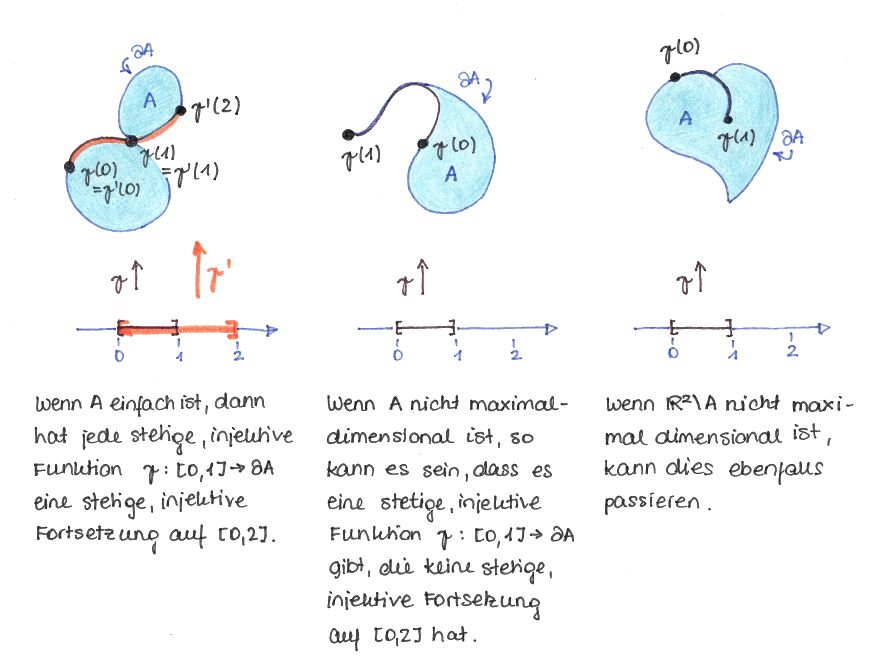
\includegraphics[width=\textwidth]{abb/rand-geht-weiter.png}
        \caption{Zu Hypothese \ref{hyp:rand-geht-weiter}}
        \label{fig:rand-geht-weiter}
    \end{figure}
%
%
%     In welchem Sinn sind einfach offene Mengen im $\R^n$ einfach? \todo{sinnvoll in den Abschnitt integrieren}
% 
%     Aus Definition \ref{def:topMet} sehen wir dass offene Teilmengen des $\R^n$ in jedem ihrer Punkte echt $n$-dimensional sind, da jeder Punkt eine ganze $\varepsilon$-Umgebung hat, die auch in der Menge liegt, man kann also von jedem Punkt aus ein Stück in jede Richtung \glqq gehen\grqq ohne die Menge zu verlassen.
%     Aus diesem Grund haben umgekehrt abgeschlossene Mengen keine niederdimensionalen Löcher. Da abgeschlossene Mengen Komplemente offener Mengen sind (Def \ref{def:CX}) ist das Komplement einer abgeschlossenen Menge überall echt $n$-dimensional.
% 
%     Wenn wir also den offene Abschluss eine Menge bilden sorgen wir durch das Abschlussbilden erst dafür, dass Löcher niederer Dimensionen verschwinden, indem wir das Innere der hierdurch entstandenen Menge nehmen schneiden wir alle niederdimensionalen Teil ab (\textcolor{red}{-> Bild}).
%     Umgekehrt werden beim abgeschlossenen Inneren erst alle Regionen der Menge entfernt, die nicht echt $n$-dimensional sind und anschließend durch den Abschluss alle niederdimensionalen Löcher.
% 
%     Dies legt nahe, dass der Rand einer einfach abgeschlossenen oder offenen Menge $n-1$-dimensional ist. Dies ist ein Frage des Dimensionsbegriffs. Man nehme Beispielsweise die Menge $M := \{(x,y) \in \R^2 \mid xy > 0\}$. Der Rand dieser Menge ist $\rand_2 M = \R \times \{0\} \cup \{0\} \times \R$ dies ist \textit{keine} 1-dimensionale topologische Mannigfaltigkeit, da es keine Umgebung des Punktes $(0,0)$ in $\rand_2 M$ gibt, die Homöomorph zu $\R$ ist.
%     
%
    \subsection{Ein Beispiel}\label{ssec:standardbsp}
    Die \strukt arbeitet mit einfachen Mengen auf den Rändern von einfachen Mengen.
    Das in Bsp.~\ref{bsp:standardbsp} eingeführte Standardbeispiel zeigt einige unerwartete Auswirkungen der Teilraumtopologie für die Einfachheit von Mengen.
    Insofern lassen sich mit seiner Hilfe möglicherweise problematische Beispiele für die im nächsten Kapitel definierten Repräsentanten konstruieren.
    Deshalb möchte ich dieses Beispiel hier näher untersuchen.
%    
    \begin{erin}\ \\
    Aus dem vorherigen Kapitel kennen wir folgende Eigenschaften der Menge %$A$ 
    \begin{align*}
        A = \bigcup_{n \in \N} [2^{-2n}, 2^{-2n+1}]
    \end{align*}
    aus Beispiel~\ref{bsp:standardbsp}:
%
        \begin{enumerate}
%             \item Die Menge $A$ aus Bsp.~\ref{bsp:standardbsp} ist definiert als
%                 \begin{align*}
%                     A := \bigcup_{n \in \N} [2^{-2n}, 2^{-2n+1}].
%                 \end{align*}
            \item Ihr Rand, Abschluss und Kern sind gegeben durch
                \begin{align*}
                    \rand A &= \{\frac{1}{2^n} \mid n \in \N\} \cup \{0\}\\
                    \cl(A) &= A \cup \{0\}\\
                    \op(A) &= \bigcup_{n \in \N} (2^{-2n}, 2^{-2n+1}).
                \end{align*}
            \item Für Mengen $M$ auf dem Rand von $A$ gilt:
                \begin{itemize}
                    \item $M$ ist abgeschlossen, falls es die $0$ enthält oder \textit{keine} Häufungspunkte hat.
                    \item $M$ ist offen, falls es die $0$ \textit{nicht} enthält oder $\rand A \setminus M$ \textit{keine} Häufungspunkte hat.
                \end{itemize}
            \item Sowohl $A$ als auch $\R \setminus A$ haben $0$ als Häufungspunkt.
            \item $\rand A$ hat $0$ als einzigen Häufungspunkt.
        \end{enumerate}
    \end{erin}
%
    Wie
    \marginpar{Einfachheit von $A$}
    sieht es mit der Einfachheit von $A$ aus?
    Es gelten:
    \begin{align*}
        &\cl(\op(\cl(A))) 
        = \cl(\op(A \cup \{0\})) 
        \\
        &\quad = \cl(\op(\bigcup_{n \in \N} [2^{-2n}, 2^{-2n+1}] \cup \{0\})) 
        = \cl(\bigcup_{n \in \N} (2^{-2n}, 2^{2n+1})) 
        \\
        &\quad = \bigcup_{n \in \N} [2^{-2n}, 2^{-2n+1}] \cup \{0\} 
        = A \cup \{0\} 
        = \cl(A)
        \\
        &\op(\cl(\op(A))) 
        = \op(\cl(\bigcup_{n \in \N} (2^{-2n}, 2^{-2n+1})))
        \\
        &\quad = \op(\bigcup_{n \in \N} [2^{-2n}, 2^{-2n+1}] \cup \{0\})
        = \bigcup_{n \in \N} (2^{-2n}, 2^{-2n+1})
        \\
        &\quad = \op(A).
    \end{align*}
%
    Deshalb ist $\cl(A)$ einfach abgeschlossen und $\op(A)$ einfach offen. 
    Nach Satz~\ref{satz:alt-def-einf-2} ist $A$ also einfach.

    Welche
    \marginpar{einfach abgeschlossene/offene Mengen auf dem Rand von $A$}
    Mengen auf dem Rand von $A$ einfach abgeschlossen bzw.\ offen oder auch keines von beidem sind, hängt nur von 3 Faktoren ab:
    \begin{enumerate}
        \item Ist $0$ in $B$?
        \item Hat $B$ einen Häufungspunkt?
        \item Hat $\rand A \setminus B$ einen Häufungspunkt?
    \end{enumerate}
    \noindent
    Da $\rand A$ einen Häufungspunkt bei $0$ hat, muss mindestens eine der Mengen $B$ oder $\rand A \setminus B$ dort auch einen Häufungspunkt haben.
    Deshalb gibt es nur noch 6 mögliche Fälle, die in Abbildung \ref{fig:tab-standardbsp} dargestellt sind.
%    
    \begin{figure}[ht]
        \centering
        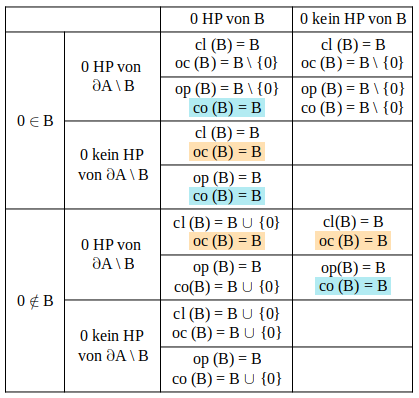
\includegraphics[width=0.7\textwidth]{abb/tab-standardbsp.png}
        \caption{Innerer Abschluss und abgeschlossenes Inneres für verschiedene Teilmengen auf $\rand A$}
        \label{fig:tab-standardbsp}
    \end{figure}
%    
%     \vspace{8pt}
%    
%     \noindent
%     \small
%     %\begin{tabularx}{\textwidth}{| p{1cm} | c | c | c | c |}
%     \begin{tabularx}{14.3cm}{| p{1cm} | c | c | c | c |}
%         \hline
%         & \multicolumn{2}{c |}{$0 \in B$} & \multicolumn{2}{c |}{$0 \notin B$}\\
%         \cline{2-5}
%         & $0$ HP von $B$ & $0$ nicht HP von $B$ & $0$ HP von $B$ & $0$ nicht HP von $B$\\
%         \hline
%         %\multirow{4}{*}{0 HP von \newline $\rand A \setminus B$}
%         \parbox[t]{2mm}{\multirow{4}{*}{\rotatebox[origin=c]{90}{\makecell{$0$ HP von\\$\rand A \setminus B$}}}}
%             & $\cl(B) = B$
%             & $\cl(B) = B$
%             & $\cl(B) = B \cup \{0\}$
%             & $\cl(B) = B$
%             \\
%             & $\oc(B) = B \setminus \{0\}$
%             & $\oc(B) = B \setminus \{0\}$
%             & $\oc(B) = B$
%             & $\oc(B) = B$
%             \\ \cline{2-5}
%             & $\op(B) = B \setminus \{0\}$
%             & $\op(B) = B \setminus \{0\}$
%             & $\op(B) = B$
%             & $\op(B) = B$
%             \\
%             & $\co(B) = B$
%             & $\co(B) = B \setminus \{0\}$
%             & $\co(B) = B \cup \{0\}$
%             & $\co(B) = B$\\
%         \hline
%         %\multirow{4}{*}{0 HP von \newline $\rand A \setminus B$}
%         %\multirow{4}{*}{\makecell{0 HP von \\ $\rand A \setminus B$}}
%         \parbox[t]{2mm}{\multirow{4}{*}{\rotatebox[origin=c]{90}{\makecell{$0$ kein \\ HP von \\ $\rand A \setminus B$}}}}
%             & $\cl(B) = B$
%             & 
%             & $\cl(B) = B \cup \{0\}$
%             & 
%             \\
%             & $\oc(B) = B$
%             & 
%             & $\oc(B) = B \cup \{0\}$
%             & 
%             \\ \cline{2-5}
%             & $\op(B) = B$
%             & 
%             & $\op(B) = B$
%             & 
%             \\
%             & $\co(B) = B$
%             & 
%             & $\co(B) = B \cup \{0\}$
%             & \\
%         \hline
%     \end{tabularx}
%     \vspace{8pt}
%     \normalsize
%    
%    \noindent
    Damit sind in $\rand A$ Teilmengen $B$
    \begin{itemize}
        \item einfach abgeschlossen, falls $0$ in $B$ und ein Häufungspunkt von $B$ oder falls $0$ \textit{nicht} in $B$ und \textit{kein} Häufungspunkt von $B$ ist
        \item einfach offen, falls $0$ in $B$ und \textit{kein} Häufungspunkt von $\rand A \setminus B$ oder falls $0$ \textit{nicht} in $B$ und ein Häufungspunkt von $\rand A \setminus B$ ist.
    \end{itemize}
%    
    \noindent
    Mit
    \marginpar{Einfachheit von Mengen und Teilraumtopologie}
    Hilfe der Menge $A$ können wir zeigen, dass es durchaus einen Unterschied für die Einfachheit von Mengen macht, auf dem Rand welcher einfachen Mengen sie liegen.
    Mit anderen Worten: Es kann einfache Mengen $A_1$ und $A_2$ geben und eine Menge, die einfach ist in $\rand A_1$, nicht jedoch in $\rand A_2$.
%
    \begin{bsp}
         Seien $A_1 := [0,1]$, $A_2 := \cl(A)$.
         Es gilt: sowohl $A_1$ als auch $A_2$ sind einfach abgeschlossen in $\R$. 
         Die Menge $B := \{0\}$ ist dann einfach abgeschlossen und einfach offen in $\rand A_1$, nicht jedoch in $\rand A_2$.
         Dort ist sie nicht einmal einfach, denn $\op_{\rand A_2} (B) = \varnothing$. D.\,h.\ $\co_{\rand A_2}(B) = \varnothing$ und somit keine Obermenge von $B$. Folglich ist nach Satz~\ref{satz:alt-def-einf-2} $B$ nicht einfach in $\rand A_2$.
    \end{bsp}

    
                            %%%%%%%%%%%%%%%%%%%%%%%%%%
                          %%%                        %%%
%%%%%%%%%%%%%%%%%%%%%%%%%%%    Spezielle Randpunkte    %%%%%%%%%%%%%%%%%%%%%%%%%%%%%%%%%%
                          %%%                        %%%
                            %%%%%%%%%%%%%%%%%%%%%%%%%%
    
\section{Äußerer Rand}\label{sec:aeusserer-rand}

    Einfache
    \marginpar{Probleme mit den Rändern einfacher Mengen}
    Mengen sind mit weiteren Einschränkungen die Kandidaten für Raumregionen. Euklidische Flächen sind einfache Mengen auf dem Rand einfacher Mengen.
    Nicht jede einfache Teilmenge des Randes jeder einfachen Teilmenge eignet sich jedoch als euklidische Fläche im Sinne der Theorie $\theoryBSO$, wie folgendes, um eine Dimension reduziertes Beispiel verdeutlicht:
%
    \begin{gegenbsp}\label{gegenbsp:aeusserer-rand}
        Seien $A := \{(x,y) \in \R^2 \mid xy > 0\}$, $B := [-1,1] \times \{0\}$ und $p := (0,0)$. 
        %Dann sind $A \in \CO(\R^2)$, $B \in \CO(\rand A)$ und $p \in \rand_{\rand A}B$.
        Dann sind $A \in \OC(\R^2)$ und $B \subseteq \rand A$.
        $p$ ist ein Randpunkt von $B$ in $\rand A$, denn $\rand A$ besteht aus der $x$- und der $y$-Achse und in jeder Umgebung von $p$ in $\rand A$ liegen sowohl Punkte der $x$-Achse, die im Inneren von $B$ sind, als auch Punkte der $y$-Achse, die nicht in $B$ sind (siehe Abbildung \ref{fig:kein-aeusserer-rand}).
        Allerdings eignet sich $p$ nicht als Grenzpunkt von $B$, denn für $p$ lässt sich nicht eindeutig eine Richtung festlegen, \glqq aus der die durch $p$ begrenzte Linie kommt\grqq, denn $B$ erstreckt sich sowohl links als auch rechts von $p$.
        Die Endpunkte $(-1,0)$ und $(1,0)$ von $B$ hingegen bezeichne ich als äußeren Rand.
    \end{gegenbsp}
%    
    \begin{figure}[ht]
        \centering
        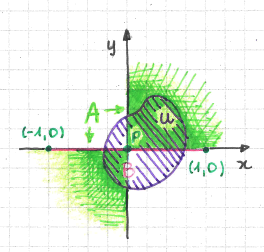
\includegraphics[width=5cm]{abb/kein-aeusserer-rand.png}
        %\caption[Kein äußerer Randpunkt]{Zu Gegenbeispiel \ref{gegenbsp:aeusserer-rand}}
        \caption{Zu Gegenbeispiel \ref{gegenbsp:aeusserer-rand}}
        \label{fig:kein-aeusserer-rand}
    \end{figure}
%
    Die
    \marginpar{äußerer Rand}
    folgende Definition formalisiert diese intuitive Vorstellung des äußeren Randes.
    Vereinfacht gesagt ist ein äußerer Randpunkt einer einfachen Menge, die auf dem Rand einer anderen einfachen Menge \glqq lebt\grqq, ein Punkt, der immer Randpunkt ist, egal, wie diese andere einfache Menge genau aussieht.
%
%     \begin{dfn}[Äußerer Rand]\label{def:aeusserer-rand} \ \vspace{8pt}
% 
%         \noindent
%         Sei $X$ ein topologischer Raum.
%         Seien $A \in \OC_X$, $B \in \OC_{\rand_X A}$ und $x \in \rand_{\rand_X A}(B)$. Dann ist $x$ ein äußerer Randpunkt von $B$, falls gilt
%         \begin{align*}
%             \forall\: A' \in \OC_X : (\: B \in \OC_{\rand_X A'} \rightarrow x \in \rand_{\rand_X A'}(B) \:)
%         \end{align*}
%         Die \thmemph{Menge der äußeren Randpunkte} von $B$ bezeichnen wir mit $\delta_X(B)$.\\
%         Ein Punkt aus $\rand_{\rand_X A} B$, der kein äußerer Randunkt von $B$ ist, heißt \thmemph{innerer Randpunkt} von $B$ in $\rand_X A$.
%     \end{dfn}
%
    \begin{dfn}[Äußerer Rand]\label{def:aeusserer-rand} \ \vspace{8pt}

        \noindent
        Sei $X$ ein topologischer Raum.
        Seien $A \in \OC_X$, $B \subseteq \rand_X A$ und $x \in \rand_{\rand_X A}(B)$. Dann ist $x$ ein äußerer Randpunkt von $B$, falls gilt
        \begin{align*}
            \forall\: A' \in \OC_X : (\: B \subseteq \rand_X A' \rightarrow x \in \rand_{\rand_X A'}(\cl_{\rand_X A'}(B)) \:)
        \end{align*}
        Die \thmemph{Menge der äußeren Randpunkte} von $B$ bezeichnen wir mit $\delta_X(B)$.\\
        Ein Punkt aus $\rand_{\rand_X A} B$, der kein äußerer Randunkt von $B$ ist, heißt \thmemph{innerer Randpunkt} von $B$ in $\rand_X A$.
    \end{dfn}
%
%
    \begin{figure}[ht]
        \centering
        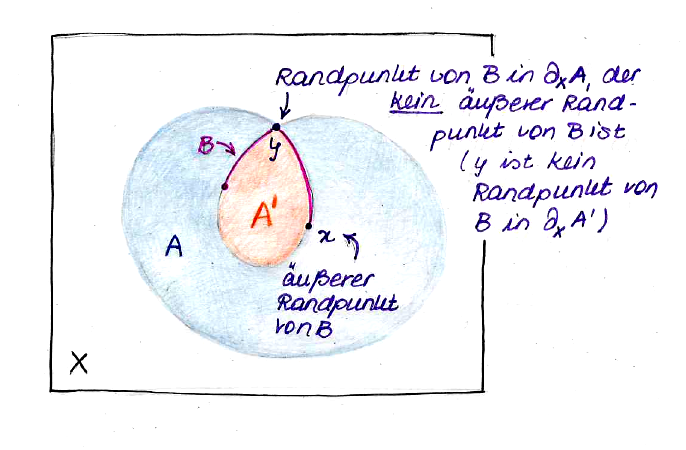
\includegraphics[height=7cm]{abb/aeusserer-rand.png}
        \caption{zu Def. \ref{def:aeusserer-rand} (äußerer Rand)}
        \label{fig:aeus-rand}
    \end{figure}
%    
    \begin{gegenbsp}\label{gegenbsp:aeusserer-rand}
       Der Punkt $p=(0,0)$ ist \textit{kein} äußerer Randpunkt von $B=[-1,1] \times \{0\}$ (siehe Gegenbeispiel \ref{gegenbsp:aeusserer-rand}), denn für $A' := \R \times \{0,\infty\} \in \OC$ ist $B \subseteq \rand A'$ aber $p$ ist keine Randpunkt von $\cl_{\rand A'} (B)$ in $\rand A'$.
    \end{gegenbsp}
%
    \begin{bsp}\label{bsp:aeusserer-rand}
        Falls die Hypothese \ref{hyp:rand-geht-weiter} stimmt, so ist
        der Punkt $q=(1,0)$ ein äußerer Randpunkt von $B=[-1,1] \times \{0\}$ (siehe Gegenbeispiel \ref{gegenbsp:aeusserer-rand}).
    \end{bsp}
%
    \begin{bew}
        Angenommen $q$ wäre kein äußerer Randpunkt von $B$.
        Dann gibt es ein $A' \in \OC$ mit $B \subseteq A'$ und $q \notin \rand_{\rand A'}(\cl_{\rand A'}(B))$.
        
        $\rand A'$ ist abgebschlossen in $\R^2$ (\ref{kor:rand-abg}), genauso wie $B$. Deshalb ist nach Korollar \ref{kor:OX-OA-CX-CA} $B$ auch in $\rand A'$ abgeschlossen und somit gilt $\cl_{\rand A'}(B) = B$.
        Also ist $q \notin \rand_{\rand A'}(B)$.
        
        Da $q \in B \subseteq \rand A'$ ist, muss es deshalb ein $V \in \offen_{\rand A'}(q)$ geben mit $V \subseteq B$.
        Sei $U \in \offen$ mit $V = U \cap \rand A'$.
        
        Sei $\gamma: [0,1] \to \rand A'$, $\gamma(t) = -1+2t$. 
        Nach Hypothese \ref{hyp:rand-geht-weiter} gibt es eine stetige injektive Abbildung $\gamma': [0,2] \to \rand A'$ mit $\gamma'(t) = \gamma(t)$ für $t \in [0,1]$.
        Da $\gamma([0,1]) = B$ ist und $\gamma'$ injektiv, ist $\gamma'(t) \notin B$ für $t \in (1,2]$.
        
        Da $\gamma'$ stetig ist und $V$ eine Umgebung von $p = \gamma'(1)$ in $\rand A'$, muss es ein $\varepsilon > 0$ geben mit $\gamma'(t) \in V$ für alle $t \in (1-\varepsilon, 1+\varepsilon)$.
        
        Also ist $\gamma'(1+\frac{\varepsilon}{2}) \in V \setminus B$, was ein Widerspruch zu $V \subseteq B$ ist. $\lightning$
    \end{bew}
%
%    
    Der
    \marginpar{äußerer Rand $n$-ter Stufe}
    Begriff des äußeren Randes lässt sich verallgemeinern zum äußeren Rand $n$-ter Stufe. Für diese Arbeit genügt uns $n = 2$.
%
    \begin{dfn}[Äußerer Rand zweiter Stufe]\label{def:aeusserer-rand-2} \ \vspace{8pt}

        \noindent
        Sei $X$ ein topologischer Raum.
        Seien $A \in \OC_X$, $B \in \OC_{\rand_X A}$, $C \subseteq \delta B$ und $x \in \rand_{\rand_{\rand_X A}(B)}(C)$. Dann ist $x$ ein äußerer Randpunkt 2.~Stufe von $C$, falls gilt:
        \begin{align*}
            &\forall\: A' \in \OC_X, B' \in \OC_{\rand_X A'} : (\: C \subseteq \delta B'\\
            &\hphantom{XXXXXXXXXXXXX} \to x \in \rand_{\rand_{\rand_X A'}(B')}(\cl_{\rand_{\rand_X A'}(B')} (C)) \:)
        \end{align*}
        Die \thmemph{Menge der äußeren Randpunkte 2. Stufe} von $C$ bezeichnen wir mit $\delta_X^2(C)$.\\
        Ein Punkt aus $\rand_{\rand_{\rand_X A}(B)}(C)$, der kein äußerer Randunkt zweiter Stufe von $C$ ist, heißt \thmemph{innerer Randpunkt} von $C$ in $\rand_{\rand_X A}(B)$.
    \end{dfn}
%    
    Die Vorstellung, die dem Begriff des äußeren Randes zugrunde liegt, ist, dass es nach einem äußeren Randpunkt \glqq wirklich nicht weiter geht\grqq.

    Im
    \marginpar{Sackgassenbild}
    $\R^2$ ist damit gemeint:
    Für eine euklidische Linie $B$ ist $p$ ein äußerer Randpunkt, wenn $B$ in $p$ eine Sackgasse hat.
    Ist dies nicht der Fall -- genauer: sind $A \in \OC_2$, $B \in \OC_{\rand A}$ und $p \in \rand_{\rand_A} B$ kein äußerer Randpunkt von $B$ -- so gibt es von $p$ aus mindestens zwei Richtungen in $B$.
    Mathematisch bedeutet dies, dass es eine stetige injektive Abbildung $\gamma:(-1,1) \to B \cup \{p\}$ gibt mit $\gamma(0) = p$.

    Die
    \marginpar{Einbettung von $\R^{n-1}$ und innere Randpunkte}
    folgende Hypothese verallgemeinert diese Vorstellungen auf Teilmengen des $\R^n$
%
    \begin{hyp}[Äußerer Rand in $\R^n$]\label{hyp:aeusserer-rand} \ \vspace{8pt}

        \noindent
        Seien $n \in \N$ mit $n \geq 2$, $A \in \einf_{\R^n}$ und $B \in \einf_{\rand_{\R^n} A}$. Ein Punkt $p \in \rand_{\rand A}(B)$ ist genau dann ein äußerer Randpunkt von $B$, falls es \textit{keine} stetige injektive Abbildung $f : U \to \cl_{\rand A}(B)$ gibt mit $p \in f(U)$ für eine offene Menge $U \in \offen_{\R^{n-1}}$.
    \end{hyp}
%    
    Diese Vorstellung gilt analog für äußere Randpunkte höherer Stufe.
    
    Die Abbildungen \ref{fig:pflasterbild-innerer-rp} und \ref{fig:pflasterbild-aeusserer-rp} illustrieren diese Hypothese für $n=3$.
    %
    \begin{figure}[ht]
        \centering
        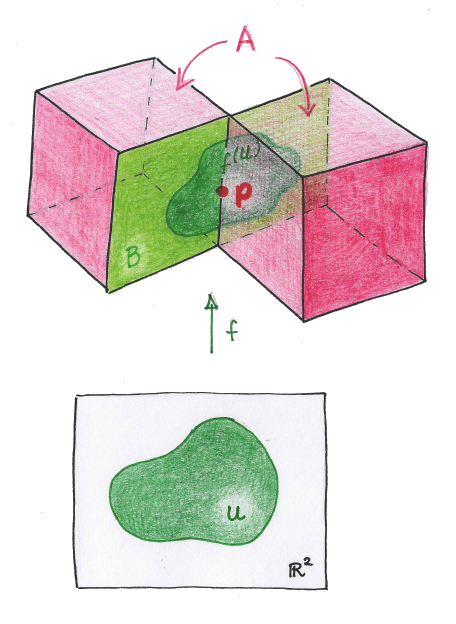
\includegraphics[height=7cm]{abb/pflasterbild-innerer-rp.png}
        \caption[Zu Hypothese \ref{hyp:aeusserer-rand} (innerer Randpunkt)]{Zu Hypothese \ref{hyp:aeusserer-rand}: Ist $p$ ein innerer Randpunkt von $B \subseteq \R^3$, so gibt es eine stetige, injektive Abbildung $f:U \to \cl_{\rand A} B$ mit $p \in f(U)$, wobei $U \in \offen_2$ ist.}
        \label{fig:pflasterbild-innerer-rp}
    \end{figure}

    \begin{figure}[ht]
        \centering
        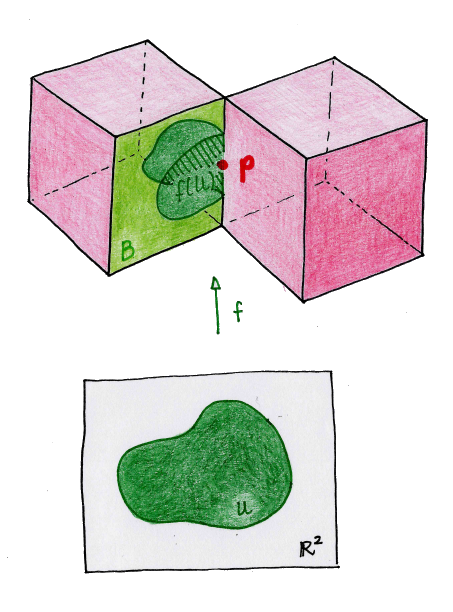
\includegraphics[height=7cm]{abb/pflasterbild-aeusserer-rp.png}
        \caption[Zu Hypothese \ref{hyp:aeusserer-rand} (äußerer Randpunkt)]{Zu Hypothese \ref{hyp:aeusserer-rand}: Ist $p$ ein äußerer Randpunkt von $B \subseteq \R^3$, so kann eine stetige Abbildung $f:U \to \cl_{\rand A} B$ mit $p \in f(U)$, wobei $U \in \offen_2$ ist, nicht injektiv sein.}
        \label{fig:pflasterbild-aeusserer-rp}
    \end{figure}
    
    Weniger
    \marginpar{Pflasterbild}
    mathematisch als in der Bildbeschreibung, kann man die Frage, ob $p$ ein äußerer Randpunkt von $B$ im $\R^3$ ist, auf folgende zurückführen:
    Ist $B$ verletzt bei $p$, kann ich dann ein Pflaster auf $B$ kleben, das $p$ überdeckt, ohne dass ich es umklappen muss (siehe Abbildungen \ref{fig:pflasterbild-aeusserer-rand} und \ref{fig:pflasterbild-innerer-pkt})?
    
    \begin{figure}[ht]
        \centering
        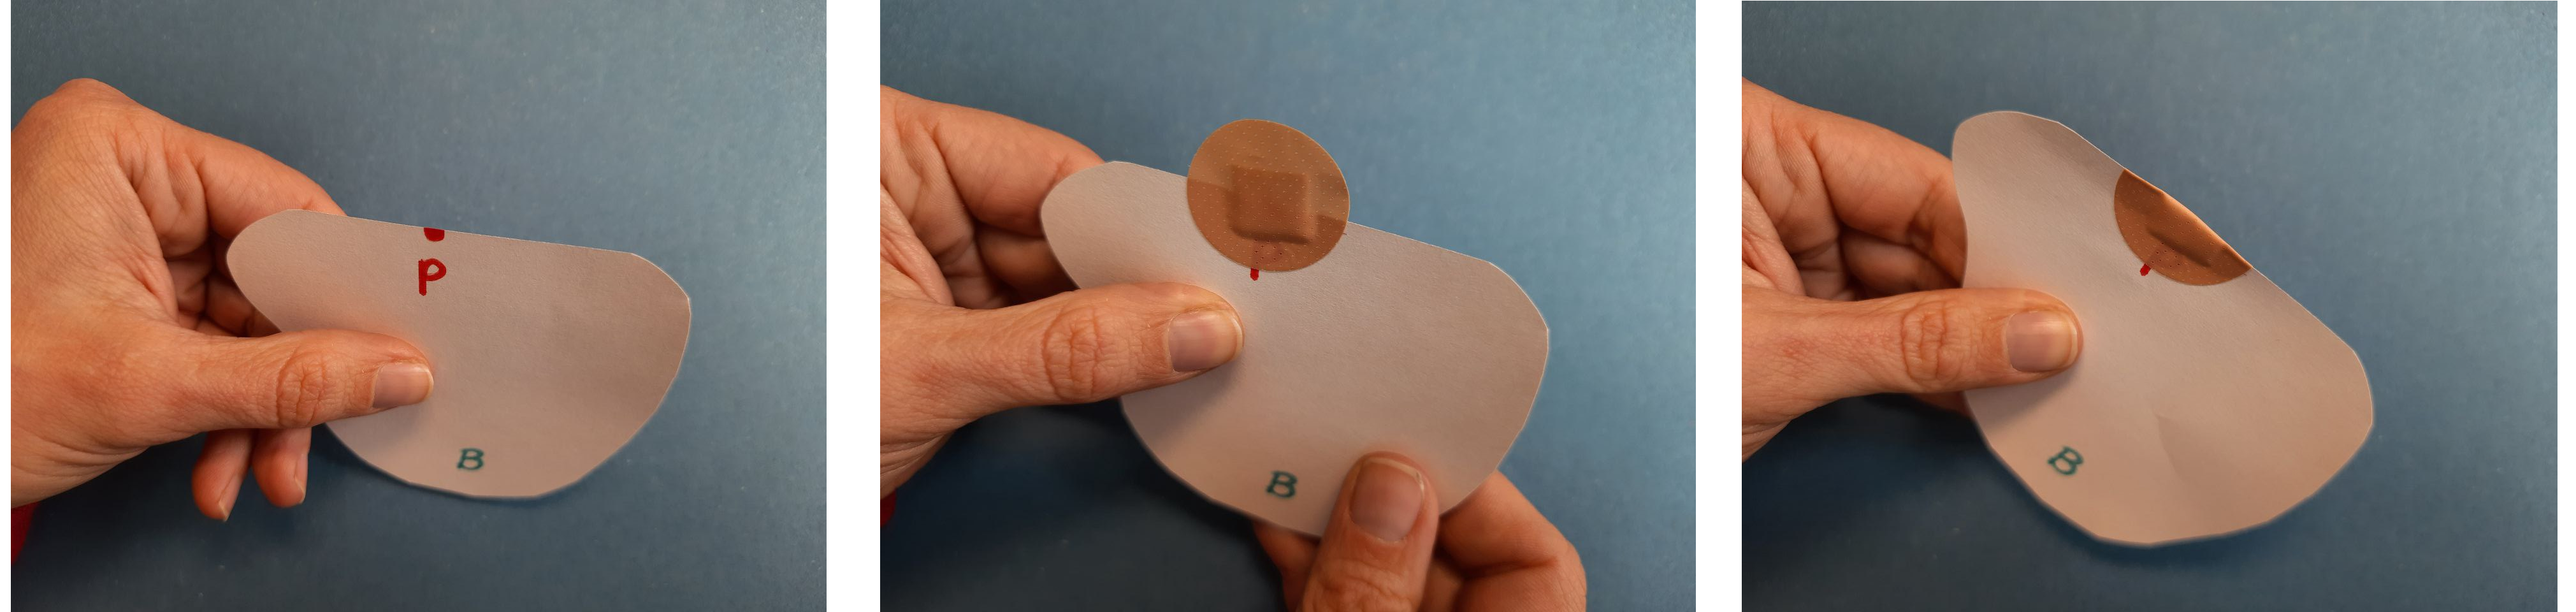
\includegraphics[width=\textwidth]{abb/pflasterbild-aeusserer-rand.png}
        \caption[Pflasterbild: äußerer Randpunkt]{Pflasterbild: Wenn $p$ ein äußerer Randpunkt einer Fläche $B$ ist, so kann ich kein Pflaster auf $B$ kleben, das $p$ überdeckt, ohne dass ich es umklappen muss.}
        \label{fig:pflasterbild-aeusserer-rand}
    \end{figure}
    
    \begin{figure}[ht]
        \centering
        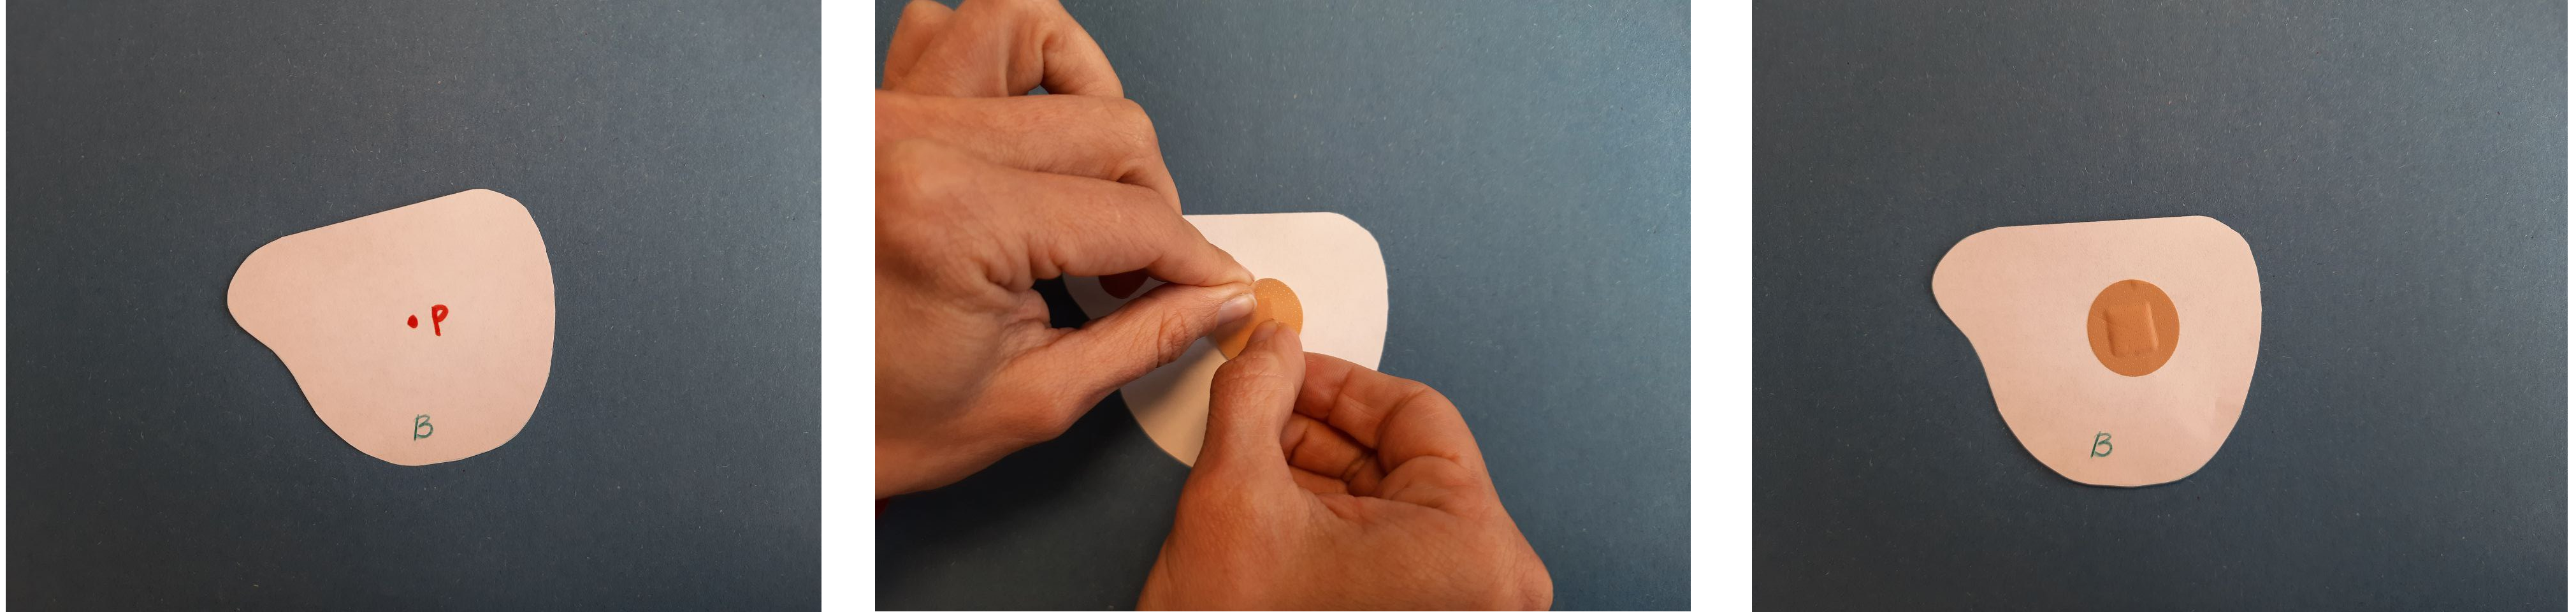
\includegraphics[width=\textwidth]{abb/pflasterbild-innerer-pkt.png}
        \caption[Pflasterbild: innerer Punkt]{Pflasterbild: Wenn $p$ ein innerer (Rand)Punkt einer Fläche $B$ ist, so kann ich ein Pflaster auf $B$ kleben, das $p$ überdeckt, ohne es umzuklappen.}
        \label{fig:pflasterbild-innerer-pkt}
    \end{figure}
    
%    \textcolor{white}{xx}

\bigskip \noindent
Mit dem äußeren Rand sowie den eingangs in diesem Kapitel eingeführten Konzepten der lokalen Gleichheit und insbesondere der einfachen Mengen sind nun zusätzliche topologische Grundlagen geschaffen. Darauf aufbauend können die Entwicklungslinien aus den vorstehenden Kapiteln dieser Arbeit in deren sich nun anschließendem dritten Teil zusammengeführt werden, um die bislang grundlegend entworfene Interpretation für die Axiomatisierung $\theoryBSO$ in der angestrebten Art und Weise weiter zu entwickeln und auf ihre Zweckmäßigkeit für den Nachweis der Konsistenz der Theorie hin zu untersuchen.

    

                            %%%%%%%%%%%%%%%%%%%%%%%%%%%%%%%
                          %%%                             %%%
%%%%%%%%%%%%%%%%%%%%%%%%%%%    Notationelle Konventionen    %%%%%%%%%%%%%%%%%%%%%%%%%%%%%%%%%%
                          %%%                             %%%
                            %%%%%%%%%%%%%%%%%%%%%%%%%%%%%%%
    
% \section{Notationelle Konventionen auf $\R^3$}\label{ssec:notationelle-konv}
% Da der hier vorgestellte Interpretationsansatz für $\BS^O$ auf einfach abgeschlossenen Mengen, derer Rändern und deren äußeren Rändern arbeitet, führe ich hierfür vereinfachte Notationen ein. Abbildung \ref{fig:notationen-r3} zeigt die eingeführten Konventionen an ausgewählten Beispielen.
% 
% \begin{figure}[ht]
%     \centering
%     \includegraphics[height=7cm]{abb/notationen-r3.png}
%     \caption{Beispiele und Gegenbeispiele zum äußeren Rand mit vereinfachter Notation}
%     \label{fig:notationen-r3}
% \end{figure}
% 
% \begin{konv}[Topologische Notationen auf $\R^3$]\ \vspace{8pt}
% 
% \noindent 
%     Im $\R^3$ vereinfachen wir die topologischen Notationen für
%     \begin{enumerate}
%     	\item die \thmemph{Topologie} $\offen_{\R^3}$ durch $\offen$
%     	\item den \thmemph{Abschlussoperator} $\cl_{\R^3}$ durch $\cl$
%     	\item den \thmemph{Kernoperator} $\op_{\R^3}$ durch $\op$
%     	\item den \thmemph{$\boldsymbol{\co}$-Operator} $\co_{\R^3}$ durch $\co$
%     	\item den \thmemph{$\boldsymbol{\oc}$-Operator} $\oc_{\R^3}$ durch $\oc$
%     	\item den \thmemph{Randoperator} $\rand_{\R^3}$ durch $\rand$
%     	%\item den \thmemph{echten Randoperator} $\Delta_{\R^3}$ durch $\Delta$
%     	\item den \thmemph{äußeren Randoperator} $\delta_{\R^3}$ durch $\delta$
%     	\item die \thmemph{Menge der einfachen Mengen} $\einf_{\R^3}$ durch $\einf$
%     	\item die \thmemph{Menge der einfach abgeschlossenen Mengen} $\CO_{\R^3}$ durch $\OC$
%     	\item die \thmemph{Menge der einfach offenen Mengen} $\OC_{\R^3}$ durch $\OC$
%     \end{enumerate}
%     
% %    \noindent
% %    Für $A \subseteq \R^3$ schreiben wir auch $\rand A$ statt $\rand (A)$.
% 
% \end{konv}
% 
% 
% \begin{konv}[Topologische Notationen auf $\rand A$]\ \vspace{8pt}
% 
% \noindent 
%     Für $A \in \CO$ vereinfachen wir die topologischen Notationen auf $\rand A$ für
%     \begin{enumerate}
%     	\item die \thmemph{Topologie} $\offen_{\rand A}$ durch $\offen_A$
%     	\item den \thmemph{Abschlussoperator} $\cl_{\rand A}$ durch $\cl_A$
%     	\item den \thmemph{Kernoperator} $\op_{\rand A}$ durch $\op_A$
%     	\item den \thmemph{$\boldsymbol{\co}$-Operator} $\co_{\rand A}$ durch $\co_A$
%     	\item den \thmemph{$\boldsymbol{\oc}$-Operator} $\oc_{\rand A}$ durch $\oc_A$
%     	\item den \thmemph{Randoperator} $\rand_{\rand A}$ durch $\rand_A$
%     	%\item den \thmemph{echten Randoperator} $\Delta_{\Delta A}$ durch $\Delta_A$
%     	\item den \thmemph{äußeren Randoperator} $\delta_{\rand A}$ durch $\delta_A$
%     	\item die \thmemph{Menge der einfachen Mengen} $\einf_{\rand A}$ durch $\einf_A$
%     	\item die \thmemph{Menge der einfach abgeschlossenen Mengen} $\CO_{\rand A}$ durch $\CO_A$
%     	\item die \thmemph{Menge der einfach offenen Mengen} $\OC_{\rand A}$ durch $\OC_A$
%     \end{enumerate}
% 
% \end{konv}
% 
% 
% % \begin{konv}[Topologische Notationen auf $\delta(B)$]\ \vspace{8pt}
% % 
% % \noindent 
% %     Für $A \in \CO$ und $B \in \CO_A$ vereinfachen wir die topologischen Notationen auf $\delta B$ für
% %     \begin{enumerate}
% %     	\item die \thmemph{Topologie} $\offen_{\Delta_A(B)}$ durch $\offen_{A,B}$
% %     	\item den \thmemph{Abschlussoperator} $\cl_{\Delta_A(B)}$ durch $\cl_{A,B}$
% %     	\item den \thmemph{Kernoperator} $\op_{\Delta_A(B)}$ durch $\op_{A,B}$
% %     	\item den \thmemph{$\boldsymbol{\co}$-Operator} $\co_{\Delta_A(B)}$ durch $\co_{A,B}$
% %     	\item den \thmemph{$\boldsymbol{\oc}$-Operator} $\oc_{\Delta_A(B)}$ durch $\oc_{A,B}$
% %     	\item den \thmemph{Randoperator} $\rand_{\Delta_A(B)}$ durch $\rand_{A,B}$
% %     	\item den \thmemph{echten Randoperator} $\Delta_{\Delta_A(B)}$ durch $\Delta_{A,B}$
% %     	\item den \thmemph{äußeren Randoperator} $\delta_{\Delta_A(B)}$ durch $\delta_{A,B}$
% %     	\item die \thmemph{Menge der einfach abgeschlossenen Mengen} $\CO_{\Delta_A(B)}$ durch $\CO_{A,B}$
% %     	\item die \thmemph{Menge der einfach offenen Mengen} $\OC_{\Delta_A(B)}$ durch $\OC_{A,B}$
% %     \end{enumerate}
% % 
% % \end{konv}
% 
